\documentclass[UTF8,a4paper,9pt]{ctexart}
\usepackage[left=1.35cm,right=1.35cm,top=0.58cm,bottom=0.48cm]{geometry}
\usepackage{xcolor,enumitem,tabularx,array,graphicx,hyperref,parskip}
\usepackage{fontawesome5}
\usepackage{tikz}
\definecolor{sjtuRed}{HTML}{B51E2A}
\definecolor{sjtuBlue}{HTML}{07539A}
\definecolor{lightBlue}{HTML}{EAF2FB}
\definecolor{grayText}{HTML}{555555}
\hypersetup{colorlinks=true,urlcolor=sjtuBlue}
\setlength{\parindent}{0pt}
\setlength{\parskip}{0pt}
\setlist[itemize]{leftmargin=1.15em,itemsep=0pt,topsep=0pt,parsep=0pt}
\newcommand{\secicon}[1]{\textcolor{sjtuBlue}{\raisebox{-0.10em}{\normalsize #1}}}
\newcommand{\sectiontitleicon}[2]{\vspace{4pt}\noindent\secicon{#1}\hspace{0.42em}{\Large\bfseries\color{sjtuBlue}#2}\vspace{1pt}\par}
\newcommand{\sectiontitle}[1]{\sectiontitleicon{\faList}{#1}}
\newcommand{\entry}[3]{\vspace{0.5pt}\textbf{#1}\hfill\textbf{\color{grayText}#3}\\[-1pt]{\color{grayText}#2}\par\vspace{0.5pt}}
\newcommand{\skill}[2]{\textbf{#1}#2\par}
\begin{document}
\pagestyle{empty}
\pagecolor{lightBlue}
% Header geometry follows the reference: blue side blocks align to the gray bar,
% and the photo floats above that bar without covering the name.
\begin{tikzpicture}[remember picture,overlay]
  \fill[white] ([xshift=.52cm,yshift=-.52cm]current page.north west) rectangle ([xshift=-.52cm,yshift=.52cm]current page.south east);
  \fill[gray!12] ([xshift=.52cm,yshift=-2.75cm]current page.north west) rectangle ([xshift=-.52cm,yshift=-4.35cm]current page.north east);
  \fill[sjtuBlue] ([xshift=.52cm,yshift=-2.75cm]current page.north west) rectangle ([xshift=1.55cm,yshift=-4.35cm]current page.north west);
  \fill[sjtuBlue] ([xshift=-.52cm,yshift=-2.75cm]current page.north east) rectangle ([xshift=-1.55cm,yshift=-4.35cm]current page.north east);
  \node[anchor=north west,inner sep=0pt] at ([xshift=1.18cm,yshift=-.92cm]current page.north west){
\includegraphics[width=5.0cm]{sjtu_brand_cropped.png}};
  % Name is right-aligned immediately against the photo's upper-left edge.
  % Center the name vertically in the white band between the page border and gray bar.
  \node[anchor=east,inner sep=0pt] at ([xshift=16cm,yshift=-1.64cm]current page.north west){{\fontsize{26}{28}\selectfont\bfseries\color{sjtuBlue}克劳德}};
  % Contact details fill the gray area to the left of the photo in two aligned columns.
  \node[anchor=west,align=left,font=\fontsize{12}{18}\selectfont] at ([xshift=1.7cm,yshift=-3.6cm]current page.north west){\textbf{电话：}xxxxxxxxxxx\\[1pt]\textbf{邮箱：}xxxxxx@sjtu.edu.cn};
  \node[anchor=west,align=left,font=\fontsize{12}{18}\selectfont] at ([xshift=11.5cm,yshift=-3.6cm]current page.north west){\textbf{出生日期：}20xx.xx.xx\\[1pt]\textbf{政治面貌：}中共党员};
  \fill[blue!8] ([xshift=16.2cm,yshift=-.8cm]current page.north west) rectangle ([xshift=18.8cm,yshift=-4.4cm]current page.north west);
  \draw[white,line width=1pt] ([xshift=16.2cm,yshift=-.8cm]current page.north west) rectangle ([xshift=18.8cm,yshift=-4.4cm]current page.north west);
  \node[inner sep=0pt] at ([xshift=17.5cm,yshift=-2.6cm]current page.north west){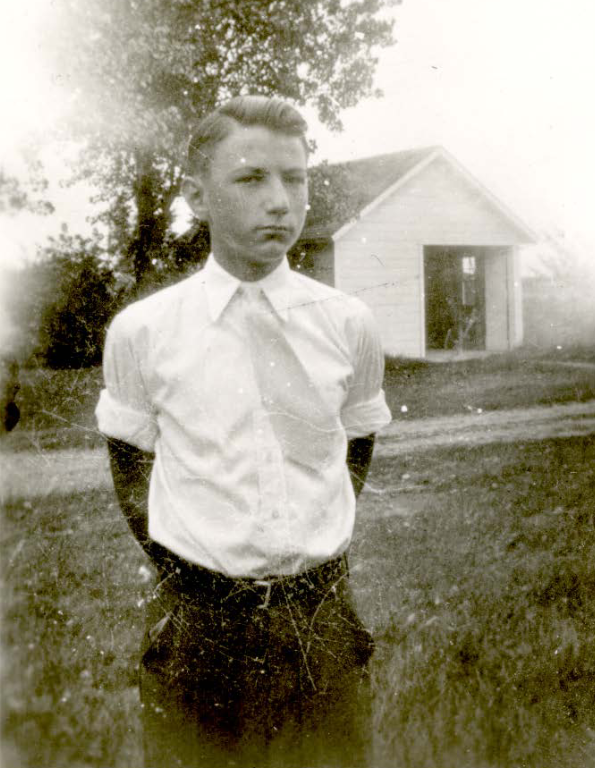
\includegraphics[width=2.5cm,height=3.5cm]{claude_shannon.png}};
\end{tikzpicture}
\vspace*{3.38cm}

\sectiontitleicon{\faGraduationCap}{教育经历}
\entry{上海交通大学（SJTU）}{信息安全 · 本科}{xxxx.xx-xxxx.xx}

\sectiontitleicon{\faCogs}{AI 技能概览}
\skill{Agent 与大模型：}{ReAct、Plan-and-Solve、多 Agent 协同、动态 Prompt、多轮状态管理、Function Calling / Tool Use。}
\skill{RAG 与工具链：}{知识库解析与向量化、语义检索、知识图谱、MCP 工具设计、意图识别、Chain-of-Thought 推理。}
\skill{工程实现：}{Python/C++、AST 解析、静态分析、自动修复、CI/CD 集成；熟悉 CodeAgent（OpenCode）框架。}

\sectiontitleicon{\faBriefcase}{AI 工作经历}
\entry{xxx}{通用软件开发工程师（AI方向）}{xxxx.xx-至今}
\begin{itemize}
\item 参与企业级智能助手建设，负责 Agent 流程编排与工具接入，支持需求拆解、检索和结果生成。
\item 使用 Python 完成数据清洗、知识库整理和效果评测，沉淀可复用的提示词与交互流程。
\end{itemize}

\sectiontitleicon{\faLayerGroup}{AI 项目经历}
\entry{企业知识问答助手}{文档检索与智能问答应用}{xxxx.xx-xxxx.xx}
\begin{itemize}
\item 完成 PDF、Markdown 等资料的切分、向量化与召回，搭建可追溯的 RAG 问答链路。
\item 增加引用定位、问题改写和多轮上下文能力，改善复杂问题的回答稳定性。
\end{itemize}
\entry{智能编码工作台}{从需求到代码的辅助开发工具}{xxxx.xx-xxxx.xx}
\begin{itemize}
\item 设计需求解析、代码生成与测试建议三个模块，支持常见开发任务的自动化流转。
\item 接入代码检索、格式检查和单元测试工具，形成可回溯的生成记录与人工确认环节。
\end{itemize}
\entry{团队协作机器人}{消息触发的任务与摘要服务}{xxxx.xx-xxxx.xx}
\begin{itemize}
\item 将群聊指令转换为任务、提醒和文档查询请求，提供统一的工具调用入口。
\item 实现会话状态保存、结果摘要和定时推送，减少重复的信息整理工作。
\end{itemize}
\entry{运维工单分析工具}{日志归因与历史案例检索}{xxxx.xx-xxxx.xx}
\begin{itemize}
\item 解析运行日志并关联历史案例，生成结构化摘要和初步处置建议。
\item 设计检索评测集与反馈记录，持续优化召回结果和回答模板。
\end{itemize}

\sectiontitleicon{\faUserTie}{其他经历}
\entry{xxx}{算法实习生}{xxxx.xx-xxxx.xx}
\begin{itemize}\item 算法实习：负责 iOS 美妆特效 Metal 推理加速，将 24 个算法包迁移至 GPU，完成跨端渲染对齐。\end{itemize}
\entry{xxx}{算法实习生}{xxxx.xx-xxxx.xx}
\begin{itemize}\item 算法实习：参与 Webots 仿真场景、机器人参数配置与数据集适配。\end{itemize}

\sectiontitleicon{\faTrophy}{竞赛与荣誉}
\begin{itemize}
\item xxx MCM 美国大学生数学建模大赛 M 奖（一等奖）。
\item 中国大学生服务外包创新创业大赛二等奖；第17届全国大学生信息安全竞赛优胜奖。
\end{itemize}
\end{document}
